% Options for packages loaded elsewhere
\PassOptionsToPackage{unicode}{hyperref}
\PassOptionsToPackage{hyphens}{url}
\PassOptionsToPackage{dvipsnames,svgnames,x11names}{xcolor}
%
\documentclass[
]{estat/estat}

\usepackage{amsmath,amssymb}
\usepackage{iftex}
\ifPDFTeX
  \usepackage[T1]{fontenc}
  \usepackage[utf8]{inputenc}
  \usepackage{textcomp} % provide euro and other symbols
\else % if luatex or xetex
  \usepackage{unicode-math}
  \defaultfontfeatures{Scale=MatchLowercase}
  \defaultfontfeatures[\rmfamily]{Ligatures=TeX,Scale=1}
\fi
\usepackage{lmodern}
\ifPDFTeX\else  
    % xetex/luatex font selection
    \setmainfont[]{Arial}
\fi
% Use upquote if available, for straight quotes in verbatim environments
\IfFileExists{upquote.sty}{\usepackage{upquote}}{}
\IfFileExists{microtype.sty}{% use microtype if available
  \usepackage[]{microtype}
  \UseMicrotypeSet[protrusion]{basicmath} % disable protrusion for tt fonts
}{}
\makeatletter
\@ifundefined{KOMAClassName}{% if non-KOMA class
  \IfFileExists{parskip.sty}{%
    \usepackage{parskip}
  }{% else
    \setlength{\parindent}{0pt}
    \setlength{\parskip}{6pt plus 2pt minus 1pt}}
}{% if KOMA class
  \KOMAoptions{parskip=half}}
\makeatother
\usepackage{xcolor}
\usepackage[left=3cm,right=2cm,top=3cm,bottom=2cm]{geometry}
\setlength{\emergencystretch}{3em} % prevent overfull lines
\setcounter{secnumdepth}{5}
% Make \paragraph and \subparagraph free-standing
\makeatletter
\ifx\paragraph\undefined\else
  \let\oldparagraph\paragraph
  \renewcommand{\paragraph}{
    \@ifstar
      \xxxParagraphStar
      \xxxParagraphNoStar
  }
  \newcommand{\xxxParagraphStar}[1]{\oldparagraph*{#1}\mbox{}}
  \newcommand{\xxxParagraphNoStar}[1]{\oldparagraph{#1}\mbox{}}
\fi
\ifx\subparagraph\undefined\else
  \let\oldsubparagraph\subparagraph
  \renewcommand{\subparagraph}{
    \@ifstar
      \xxxSubParagraphStar
      \xxxSubParagraphNoStar
  }
  \newcommand{\xxxSubParagraphStar}[1]{\oldsubparagraph*{#1}\mbox{}}
  \newcommand{\xxxSubParagraphNoStar}[1]{\oldsubparagraph{#1}\mbox{}}
\fi
\makeatother


\providecommand{\tightlist}{%
  \setlength{\itemsep}{0pt}\setlength{\parskip}{0pt}}\usepackage{longtable,booktabs,array}
\usepackage{calc} % for calculating minipage widths
% Correct order of tables after \paragraph or \subparagraph
\usepackage{etoolbox}
\makeatletter
\patchcmd\longtable{\par}{\if@noskipsec\mbox{}\fi\par}{}{}
\makeatother
% Allow footnotes in longtable head/foot
\IfFileExists{footnotehyper.sty}{\usepackage{footnotehyper}}{\usepackage{footnote}}
\makesavenoteenv{longtable}
\usepackage{graphicx}
\makeatletter
\newsavebox\pandoc@box
\newcommand*\pandocbounded[1]{% scales image to fit in text height/width
  \sbox\pandoc@box{#1}%
  \Gscale@div\@tempa{\textheight}{\dimexpr\ht\pandoc@box+\dp\pandoc@box\relax}%
  \Gscale@div\@tempb{\linewidth}{\wd\pandoc@box}%
  \ifdim\@tempb\p@<\@tempa\p@\let\@tempa\@tempb\fi% select the smaller of both
  \ifdim\@tempa\p@<\p@\scalebox{\@tempa}{\usebox\pandoc@box}%
  \else\usebox{\pandoc@box}%
  \fi%
}
% Set default figure placement to htbp
\def\fps@figure{htbp}
\makeatother

\authors{%
    Estatiano 1 \\
    Estatiano 2\\
    Estatiano 3\\
}

% escreva o nome do cliente aqui
% se for mais de um separe por \\
\client{%
    ESTAT
}
% Baixando pacotes
\RequirePackage{fancyhdr}
\RequirePackage{graphicx}

\setlength\headheight{28pt}  

\setlength{\parindent}{15pt} % Adiciona indentação nos parágrafos
\setlength{\parskip}{0pt} % Adiciona 0 espaço entro os parágrafos

\let\oldsection\section
\renewcommand\section{\clearpage\oldsection}
\makeatletter
\@ifpackageloaded{float}{}{\usepackage{float}}
\floatstyle{plain}
\@ifundefined{c@chapter}{\newfloat{quadro}{h}{loquad}}{\newfloat{quadro}{h}{loquad}[chapter]}
\floatname{quadro}{Quadro}
\floatstyle{plaintop}
\restylefloat{quadro}
\newcommand*\listofquadros{\listof{quadro}{List of Testes}}
\makeatother
\makeatletter
\@ifpackageloaded{caption}{}{\usepackage{caption}}
\AtBeginDocument{%
\ifdefined\contentsname
  \renewcommand*\contentsname{Índice}
\else
  \newcommand\contentsname{Índice}
\fi
\ifdefined\listfigurename
  \renewcommand*\listfigurename{Lista de Figuras}
\else
  \newcommand\listfigurename{Lista de Figuras}
\fi
\ifdefined\listtablename
  \renewcommand*\listtablename{Lista de Tabelas}
\else
  \newcommand\listtablename{Lista de Tabelas}
\fi
\ifdefined\figurename
  \renewcommand*\figurename{Figura}
\else
  \newcommand\figurename{Figura}
\fi
\ifdefined\tablename
  \renewcommand*\tablename{Tabela}
\else
  \newcommand\tablename{Tabela}
\fi
}
\@ifpackageloaded{float}{}{\usepackage{float}}
\floatstyle{ruled}
\@ifundefined{c@chapter}{\newfloat{codelisting}{h}{lop}}{\newfloat{codelisting}{h}{lop}[chapter]}
\floatname{codelisting}{Listagem}
\newcommand*\listoflistings{\listof{codelisting}{Lista de Listagens}}
\captionsetup{labelsep=colon}
\makeatother
\makeatletter
\makeatother
\makeatletter
\@ifpackageloaded{caption}{}{\usepackage{caption}}
\@ifpackageloaded{subcaption}{}{\usepackage{subcaption}}
\makeatother

\ifLuaTeX
\usepackage[bidi=basic]{babel}
\else
\usepackage[bidi=default]{babel}
\fi
\babelprovide[main,import]{portuguese}
\ifPDFTeX
\else
\babelfont{rm}[]{Arial}
\fi
% get rid of language-specific shorthands (see #6817):
\let\LanguageShortHands\languageshorthands
\def\languageshorthands#1{}
\usepackage{bookmark}

\IfFileExists{xurl.sty}{\usepackage{xurl}}{} % add URL line breaks if available
\urlstyle{same} % disable monospaced font for URLs
\hypersetup{
  pdftitle={Projeto Fantasma},
  pdflang={pt},
  colorlinks=true,
  linkcolor={black},
  filecolor={black},
  citecolor={black},
  urlcolor={black},
  pdfcreator={LaTeX via pandoc}}


\title{Projeto Fantasma}
\author{}
\date{}

\begin{document}
\maketitle

% Limpando tudo
\fancyhf{} 

% Ajustes do header
\fancyhead[L]{} % limpando o lado esquerdo
\fancyhead[R]{
\includegraphics[width=0.20\textwidth]{estat/imagens/estat.png}} % adicionando logo no canto direito
\renewcommand{\headrulewidth}{0pt}   % sem linha embaixo da logo

% Ajustes de fim de página
\fancyfoot[R]{\textcolor{white}{\thepage}} % Número em branco no canto direito

% Aplicando o estilo que acabamos de criar
\pagestyle{fancy} 


\labelformat{quadro}{\textbf{#1}}

\renewcommand*\contentsname{Sumário}
{
\hypersetup{linkcolor=}
\setcounter{tocdepth}{3}
\tableofcontents
}

\section{Introdução}\label{introduuxe7uxe3o}

\section{Referencial Teórico}\label{referencial-teuxf3rico}

\subsection{Média}\label{muxe9dia}

A média é a soma das observações dividida pelo número total delas, dada
pela fórmula:

\[\bar{X}=\frac{\sum\limits_{i=1}^{n}X_i}{n}\]

Com:

\begin{itemize}
\item
  \(i = 1, \, 2, \, ..., \, n\)
\item
  \(n =\) número total de observações
\end{itemize}

\subsection{Quartis}\label{quartis}

Os quartis são separatrizes que dividem o conjunto de dados em quatro
partes iguais. O primeiro quartil (ou inferior) delimita os 25\% menores
valores, o segundo representa a mediana, e o terceiro delimita os 25\%
maiores valores. Inicialmente deve-se calcular a posição do quartil:

\begin{itemize}
\item
  Posição do primeiro quartil \(P_1\): \[P_1=\frac{n+1}{4}\]
\item
  Posição da mediana (segundo quartil) \(P_2\): \[P_2 = \frac{n+1}{2}\]
\item
  Posição do terceiro quartil \(P_3\): \[P_3=\frac{3 \times (n+1)}{4}\]
\end{itemize}

Com \(n\) sendo o tamanho da amostra. Dessa forma,
\(X_{\left( P_i \right)}\) é o valor do \(i\)-ésimo quartil, onde
\(X_{\left( j \right)}\) representa a \(j\)-ésima observação dos dados
ordenados.

Se o cálculo da posição resultar em uma fração, deve-se fazer a média
entre o valor que está na posição do inteiro anterior e do seguinte ao
da posição.

\subsection{Variância}\label{variuxe2ncia}

A variância é uma medida que avalia o quanto os dados estão dispersos em
relação à média, em uma escala ao quadrado da escala dos dados. \#\#\#
Variância Populacional

Para uma população, a variância é dada por:

\[\sigma^2=\frac{\sum\limits_{i=1}^{N}\left(X_i - \mu\right)^2}{N}\]

Com:

\begin{itemize}
\item
  \(X_i =\) \(i\)-ésima observação da população
\item
  \(\mu =\) média populacional
\item
  \(N =\) tamanho da população
\end{itemize}

\subsubsection{Variância Amostral}\label{variuxe2ncia-amostral}

Para uma amostra, a variância é dada por:

\[S^2=\frac{\sum\limits_{i=1}^{n}\left(X_i - \bar{X}\right)^2}{n-1}\]

Com:

\begin{itemize}
\item
  \(X_i =\) i-ésima observação da amostra
\item
  \(\bar{X} =\) média amostral
\item
  \(n =\) tamanho da amostra
\end{itemize}

\subsection{Desvio Padrão}\label{desvio-padruxe3o}

O desvio padrão é a raiz quadrada da variância. Ele avalia o quanto os
dados estão dispersos em relação à média.

\subsubsection{Desvio Padrão
Populacional}\label{desvio-padruxe3o-populacional}

Para uma população, o desvio padrão é dado por:

\[\sigma=\sqrt{\frac{\sum\limits_{i=1}^{N}\left(X_i - \mu\right)^2}{N}}\]

Com:

\begin{itemize}
\item
  \(X_i =\) i-ésima observação da população
\item
  \(\mu =\) média populacional
\item
  \(N =\) tamanho da população
\end{itemize}

\subsubsection{Desvio Padrão Amostral}\label{desvio-padruxe3o-amostral}

Para uma amostra, o desvio padrão é dado por:

\[S=\sqrt{\frac{\sum\limits_{i=1}^{n}\left(X_i - \bar{X}\right)^2}{n-1}}\]

Com:

\begin{itemize}
\item
  \(X_i =\) i-ésima observação da amostra
\item
  \(\bar{X} =\) média amostral
\item
  \(n =\) tamanho da amostra \#\# Boxplot
\end{itemize}

O boxplot é uma representação gráfica na qual se pode perceber de forma
mais clara como os dados estão distribuídos. A figura abaixo ilustra um
exemplo de boxplot.

\begin{figure}[H]

\caption{Exemplo de boxplot}

{\centering \pandocbounded{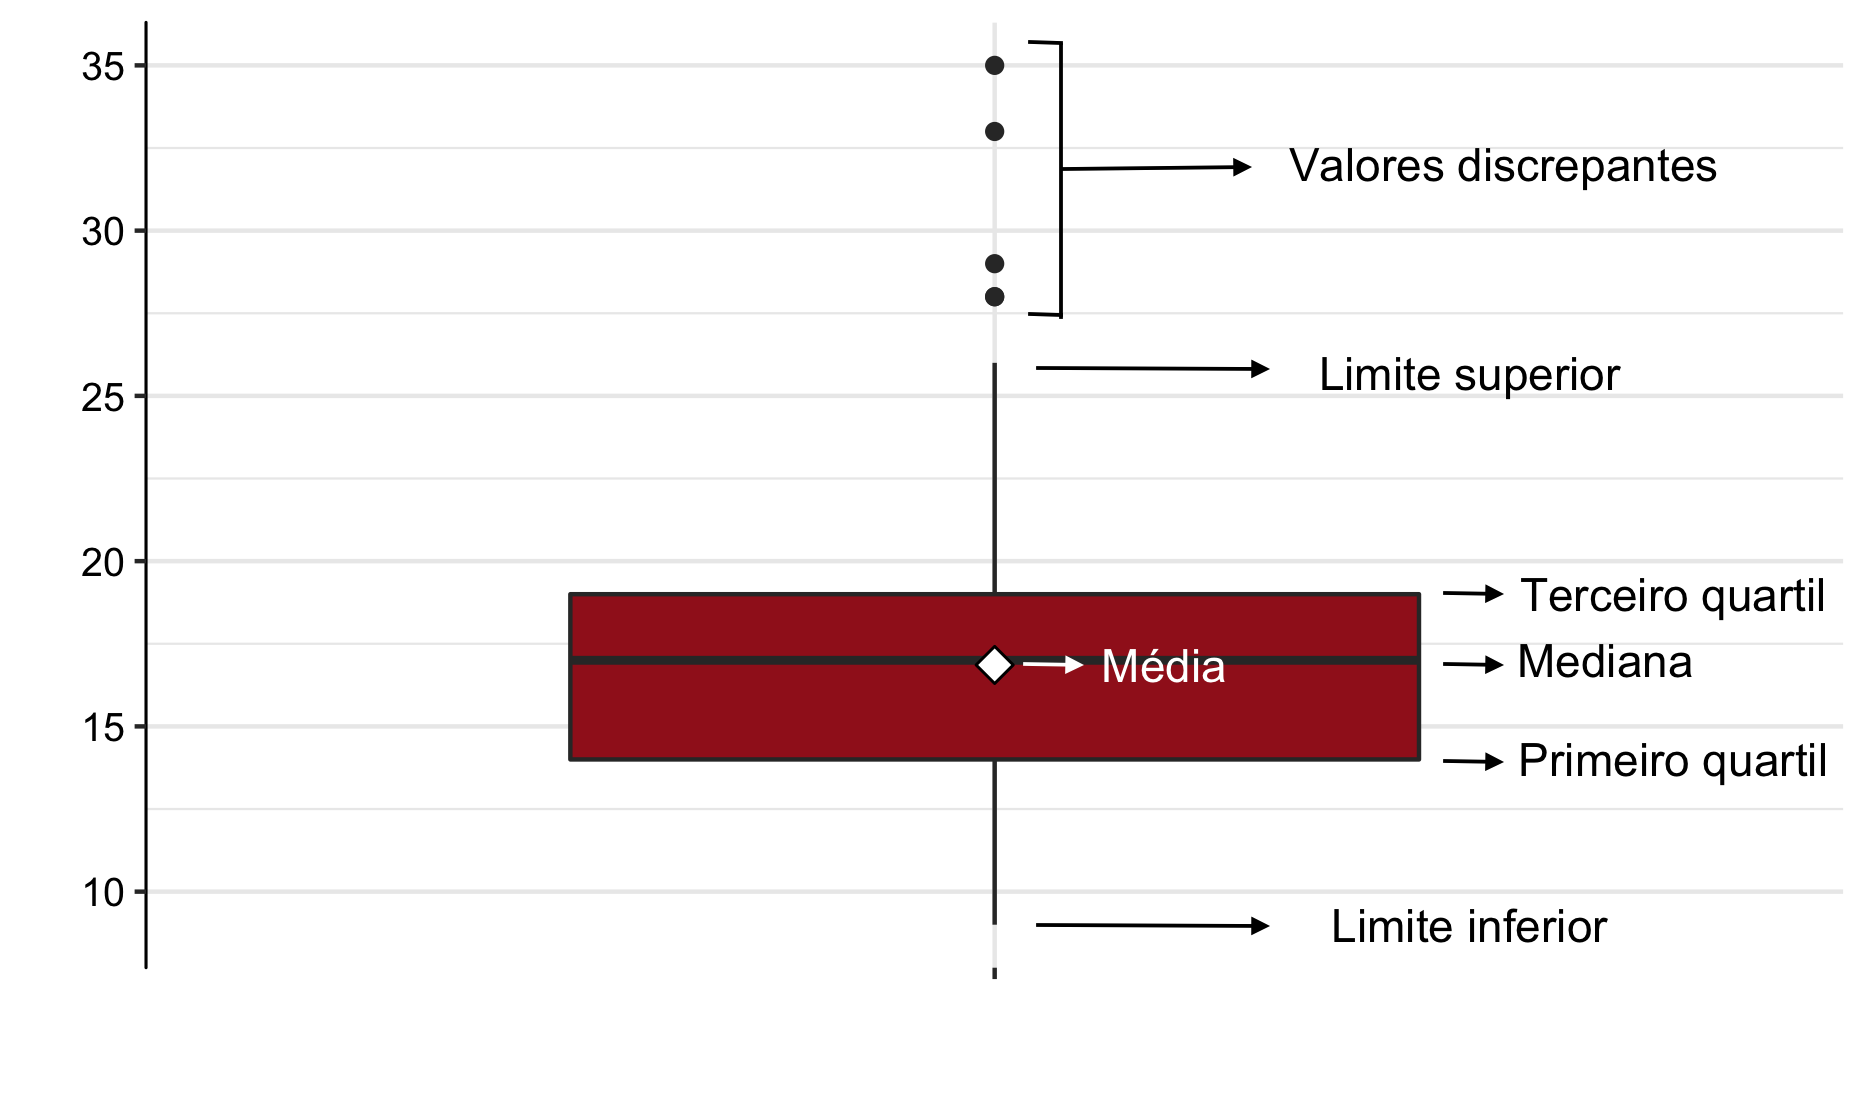
\includegraphics[keepaspectratio]{images/box_uni.png}}

}

\end{figure}%

A porção inferior do retângulo diz respeito ao primeiro quartil,
enquanto a superior indica o terceiro quartil. Já o traço no interior do
retângulo representa a mediana do conjunto de dados, ou seja, o valor em
que o conjunto de dados é dividido em dois subconjuntos de mesmo
tamanho. A média é representada pelo losango branco e os pontos são
\emph{outliers}. Os \emph{outliers} são valores discrepantes da série de
dados, ou seja, valores que não demonstram a realidade de um conjunto de
dados. \#\# Gráfico de Dispersão

O gráfico de dispersão é uma representação gráfica utilizada para
ilustrar o comportamento conjunto de duas variáveis quantitativas. A
figura abaixo ilustra um exemplo de gráfico de dispersão, onde cada
ponto representa uma observação do banco de dados.

\begin{figure}[H]

\caption{Exemplo de Gráfico de Dispersão}

{\centering \pandocbounded{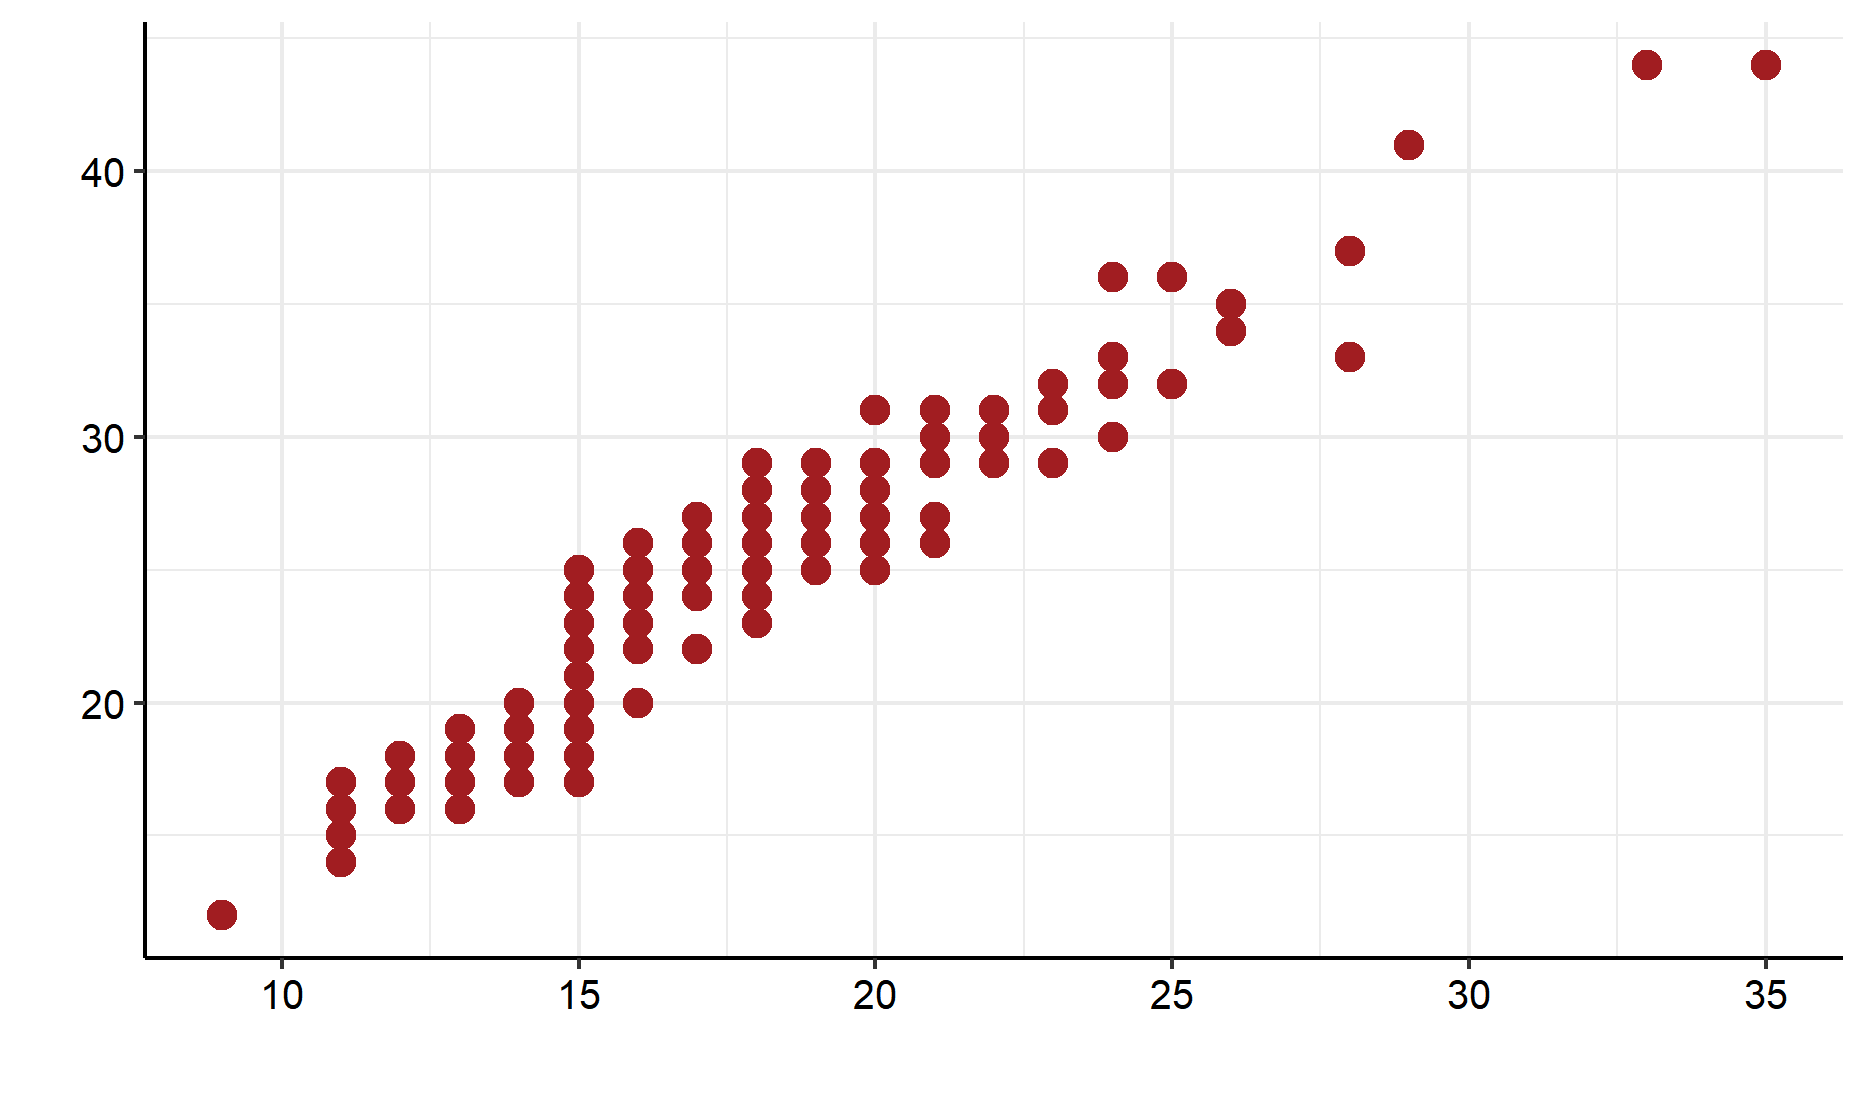
\includegraphics[keepaspectratio]{images/disp_uni.png}}

}

\end{figure}%

\subsection{Tipos de Variáveis}\label{tipos-de-variuxe1veis}

\subsubsection{Qualitativas}\label{qualitativas}

As variáveis qualitativas são as variáveis não numéricas, que
representam categorias ou características da população. Estas
subdividem-se em:

\begin{itemize}
\tightlist
\item
  \textbf{Nominais}: quando não existe uma ordem entre as categorias da
  variável (exemplos: sexo, cor dos olhos, fumante ou não, etc)
\item
  \textbf{Ordinais}: quando existe uma ordem entre as categorias da
  variável (exemplos: nível de escolaridade, mês, estágio de doença,
  etc)
\end{itemize}

\subsubsection{Quantitativas}\label{quantitativas}

As variáveis quantitativas são as variáveis numéricas, que representam
características numéricas da população, ou seja, quantidades. Estas
subdividem-se em:

\begin{itemize}
\tightlist
\item
  \textbf{Discretas}: quando os possíveis valores são enumeráveis
  (exemplos: número de filhos, número de cigarros fumados, etc)
\item
  \textbf{Contínuas}: quando os possíveis valores são resultado de
  medições (exemplos: massa, altura, tempo, etc)
\end{itemize}

\subsection{Coeficiente de Correlação de
Pearson}\label{coeficiente-de-correlauxe7uxe3o-de-pearson}

O coeficiente de correlação de Pearson é uma medida que verifica o grau
de relação linear entre duas variáveis quantitativas. Este coeficiente
varia entre os valores -1 e 1. O valor zero significa que não há relação
linear entre as variáveis. Quando o valor do coeficiente \(r\) é
negativo, diz-se existir uma relação de grandeza inversamente
proporcional entre as variáveis. Analogamente, quando \(r\) é positivo,
diz-se que as duas variáveis são diretamente proporcionais.

O coeficiente de correlação de Pearson é normalmente representado pela
letra \(r\) e a sua fórmula de cálculo é:

\[
r_{Pearson} = \frac{\displaystyle \sum_{i=1}^{n} \left [ \left(x_i-\bar{x}\right) \left(y_i-\bar{y}\right) \right]}{\sqrt{\displaystyle \sum_{i=1}^{n} x_i^2 - n\bar{x}^2}  \times \sqrt{\displaystyle \sum_{i=1}^{n} y_i^2 - n\bar{y}^2}}
\]

Onde:

\begin{itemize}
\tightlist
\item
  \(x_i =\) i-ésimo valor da variável \(X\)
\item
  \(y_i =\) i-ésimo valor da variável \(Y\)
\item
  \(\bar{x} =\) média dos valores da variável \(X\)
\item
  \(\bar{y} =\) média dos valores da variável \(Y\)
\end{itemize}

Vale ressaltar que o coeficiente de Pearson é paramétrico e, portanto,
sensível quanto à normalidade (simetria) dos dados.

\section{Análises}\label{anuxe1lises}

\subsection{Análise dos top 3 produtos mais vendidos nas top 3 lojas com
maior receita em
1889}\label{anuxe1lise-dos-top-3-produtos-mais-vendidos-nas-top-3-lojas-com-maior-receita-em-1889}

\section{Conclusões}\label{conclusuxf5es}




\end{document}
